\documentclass[a4paper, 12pt, garamond]{book}
\usepackage{cours-preambule}
\usepackage{tocloft}
\usepackage{fancybox}

\renewcommand{\mtcSfont}{\Large}
\setlength{\mtcindent}{5pt}
\mtcsetoffset{minitoc}{-5pt}
\addtolength{\cftsecnumwidth}{10pt}
\setcounter{minitocdepth}{1}

\def\lspace{25}

\dominitoc
\faketableofcontents

% \toggletrue{student}
% \toggletrue{corrige}
% \renewcommand{\mycol}{black}
% \renewcommand{\mycol}{gray}

\makeatletter
\renewcommand{\@chapapp}{MPSI3 -- 31 mai 2024 -- Devoir surveillé}
\makeatother

\setlist[blocQR,1]{leftmargin=10pt, label=\sqenumi}
\counterwithin*{equation}{section}

\begin{document}
\setcounter{chapter}{8}

% \settype{enon}
% \settype{solu_prof}
% \settype{solu_stud}

\chapter{Correction du DS}
\label{ch:ds09}

\section"E"{Étude de deux gaz parfaits dans un cylindre}

\begin{center}
	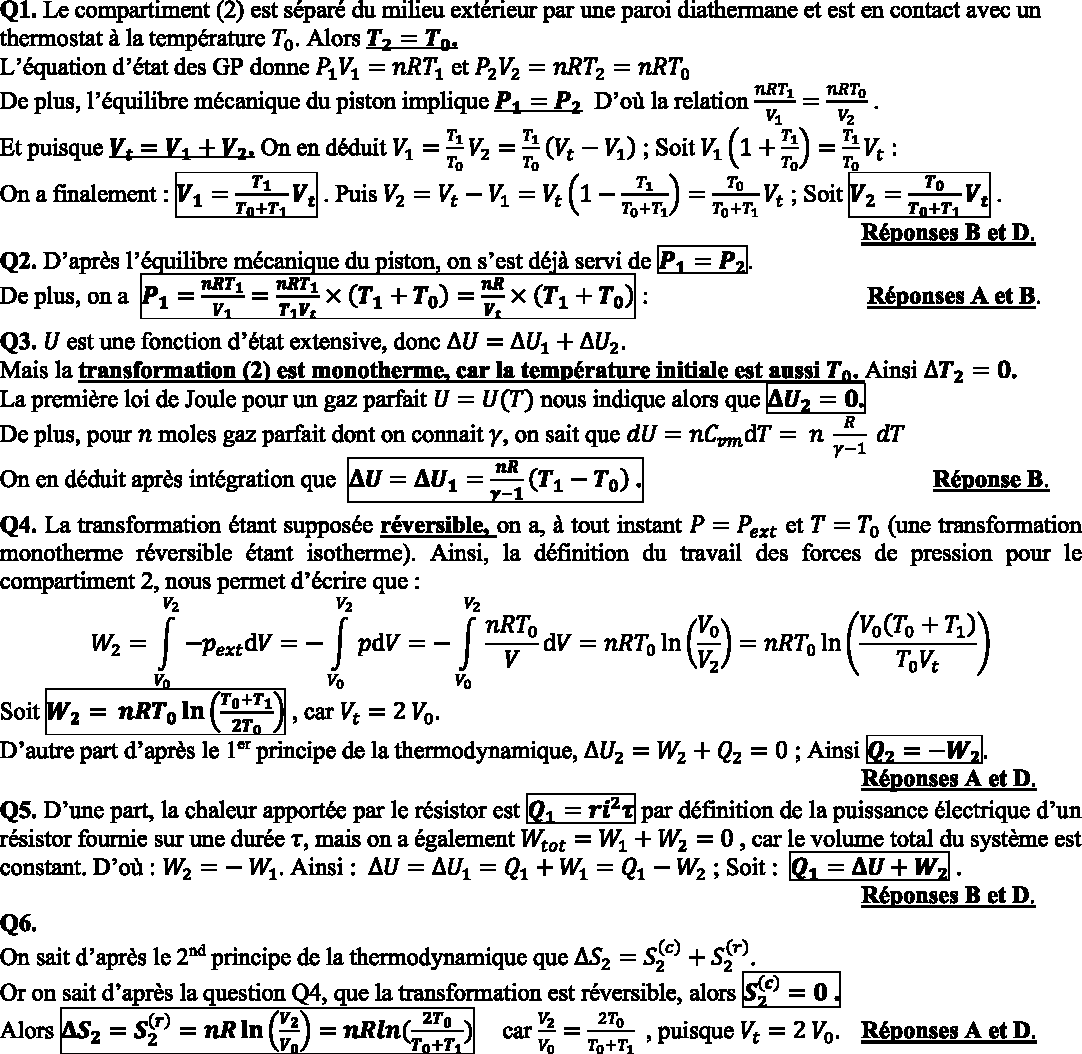
\includegraphics[width=\linewidth]{figures/pb-2gaz-corr1.pdf}
\end{center}

\section"E"{Cycle de Carnot}

\begin{center}
	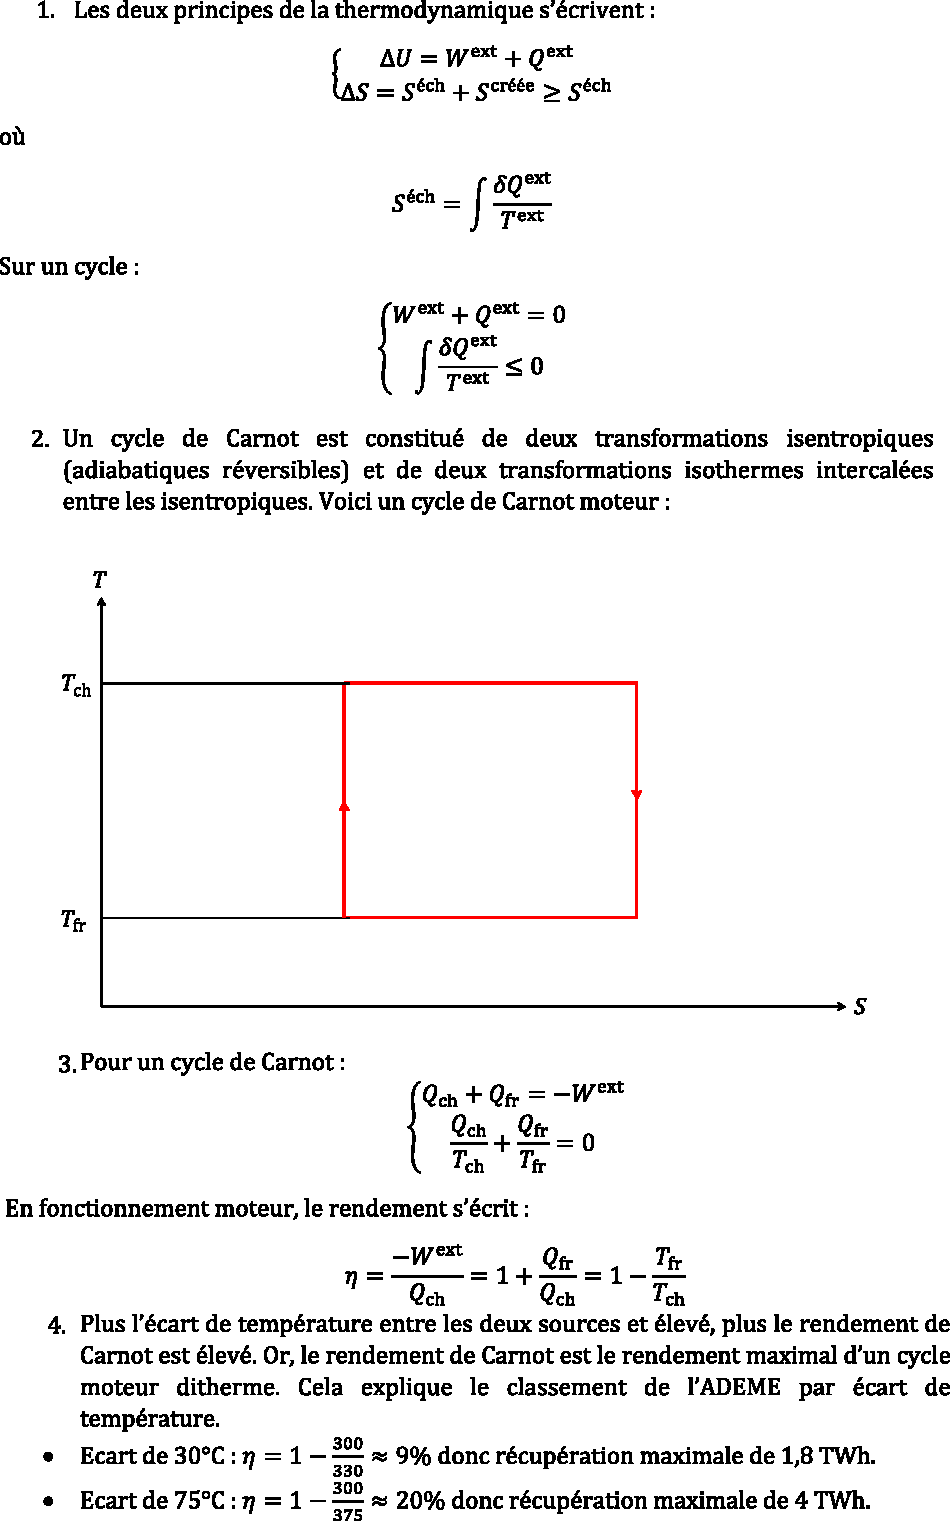
\includegraphics[width=.85\linewidth]{figures/pb-carnot-corr1.pdf}\\
	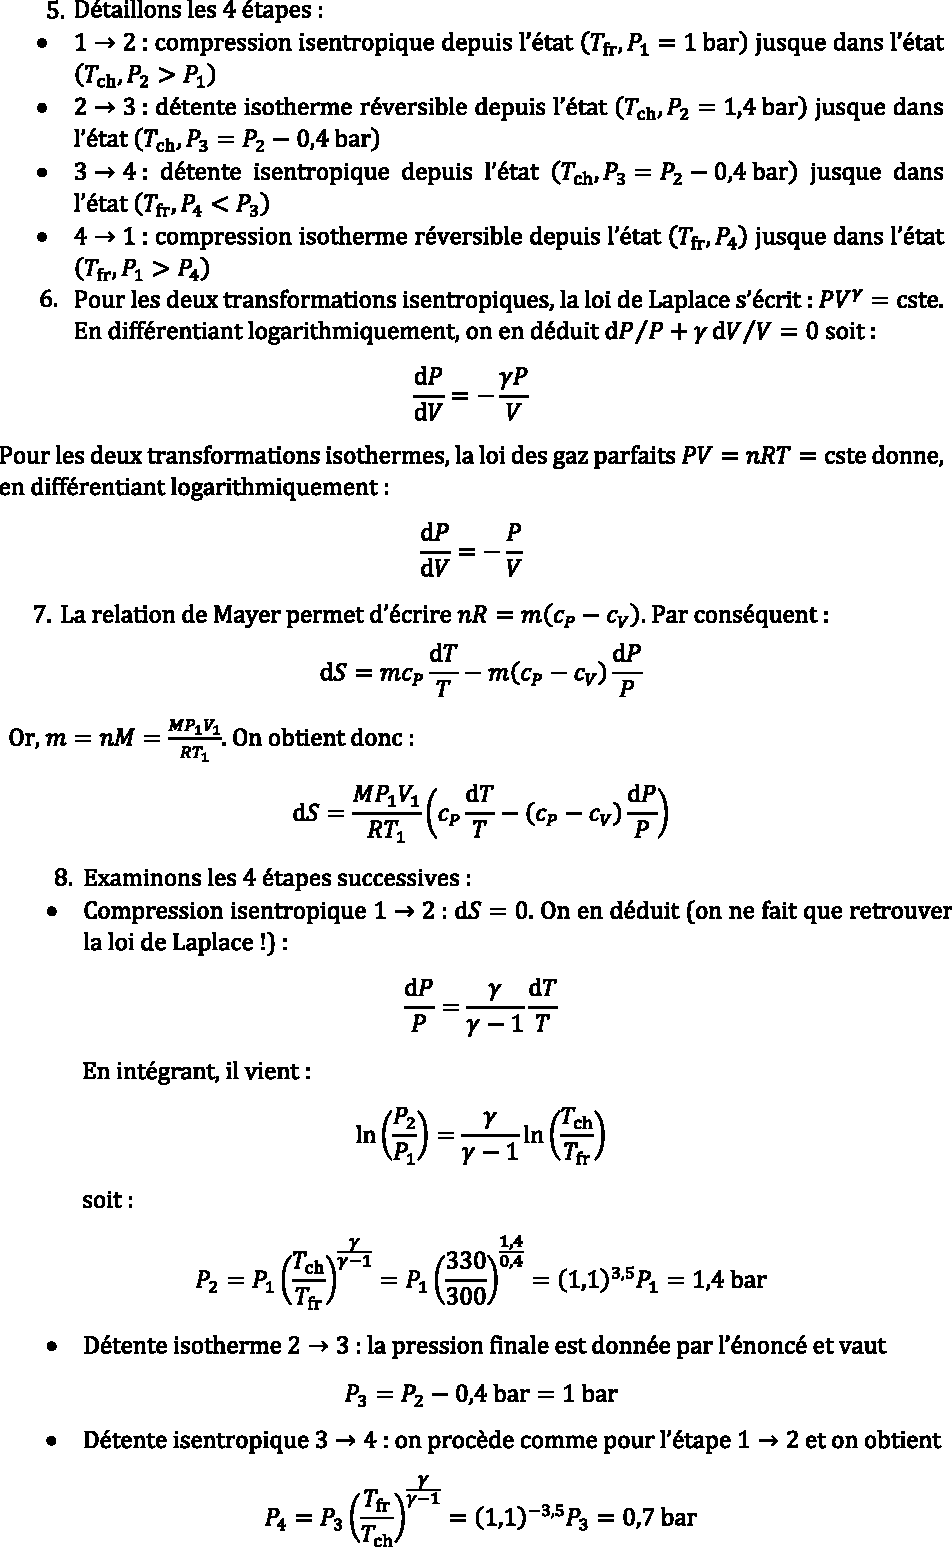
\includegraphics[width=.9\linewidth]{figures/pb-carnot-corr2.pdf}\\
	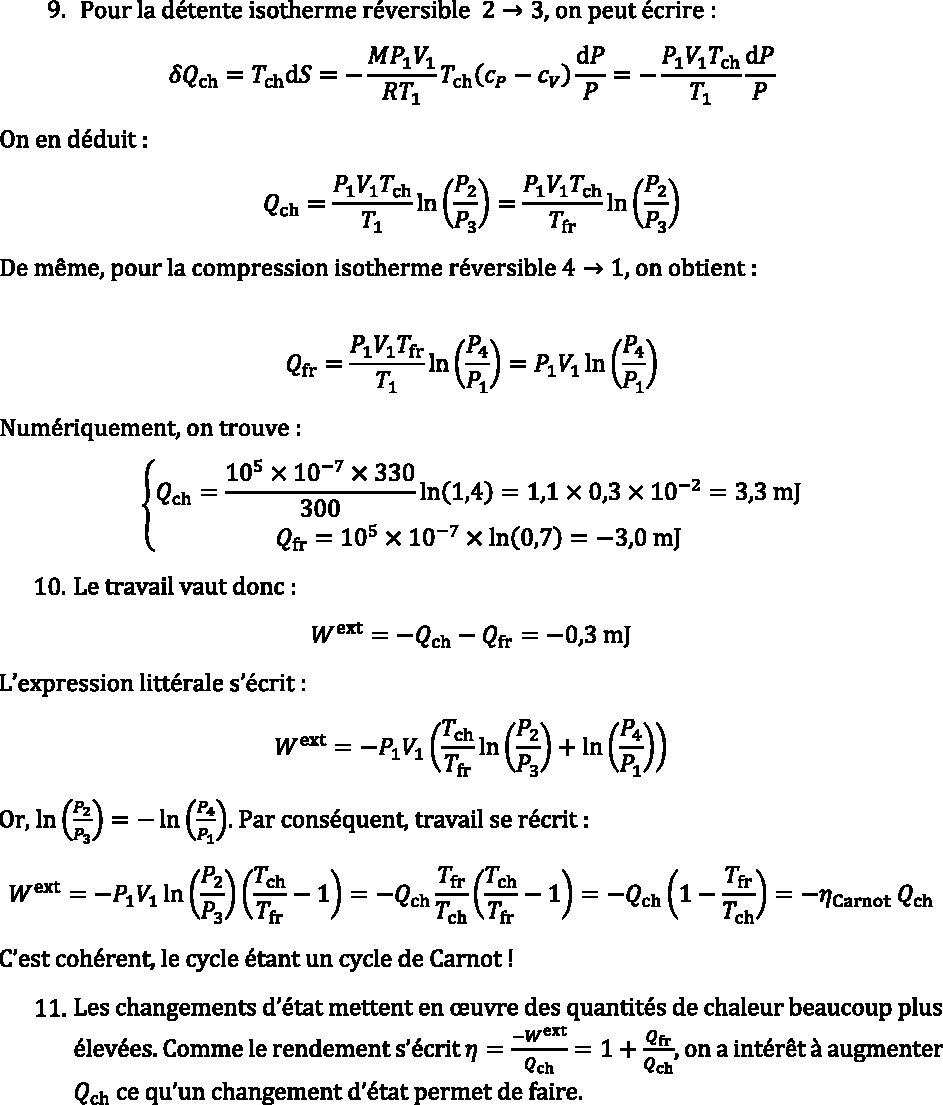
\includegraphics[width=\linewidth]{figures/pb-carnot-corr3.pdf}
\end{center}

\newpage

\section"P"{Moteur de Stirling}

\begin{center}
	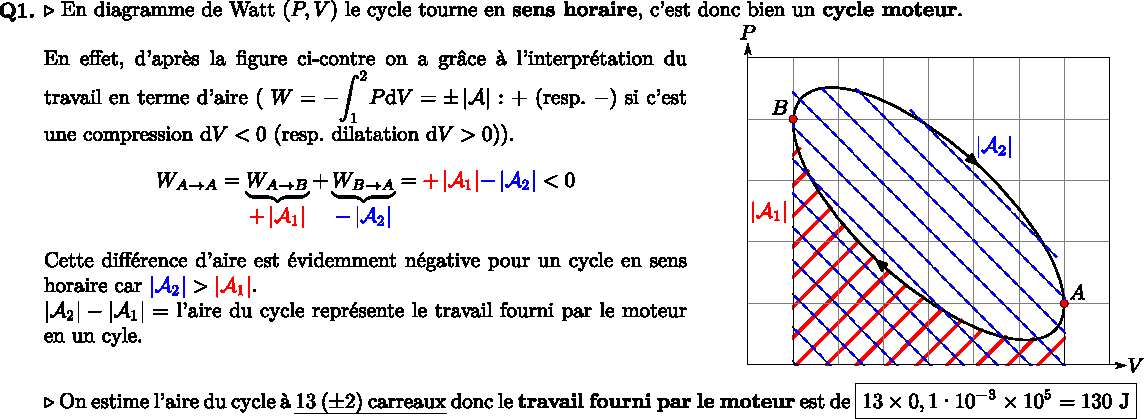
\includegraphics[width=\linewidth]{figures/pb-stirling-corr1.pdf}\\
	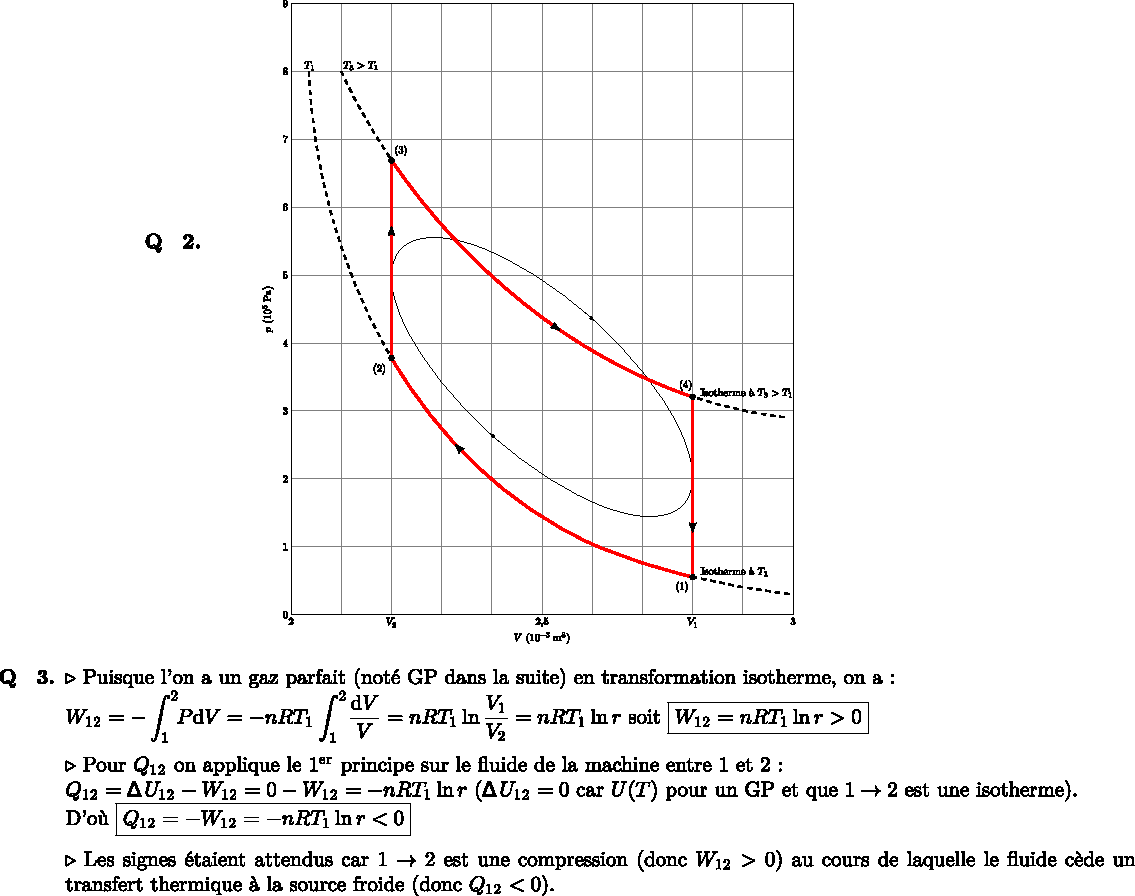
\includegraphics[width=\linewidth]{figures/pb-stirling-corr2.pdf}\\
	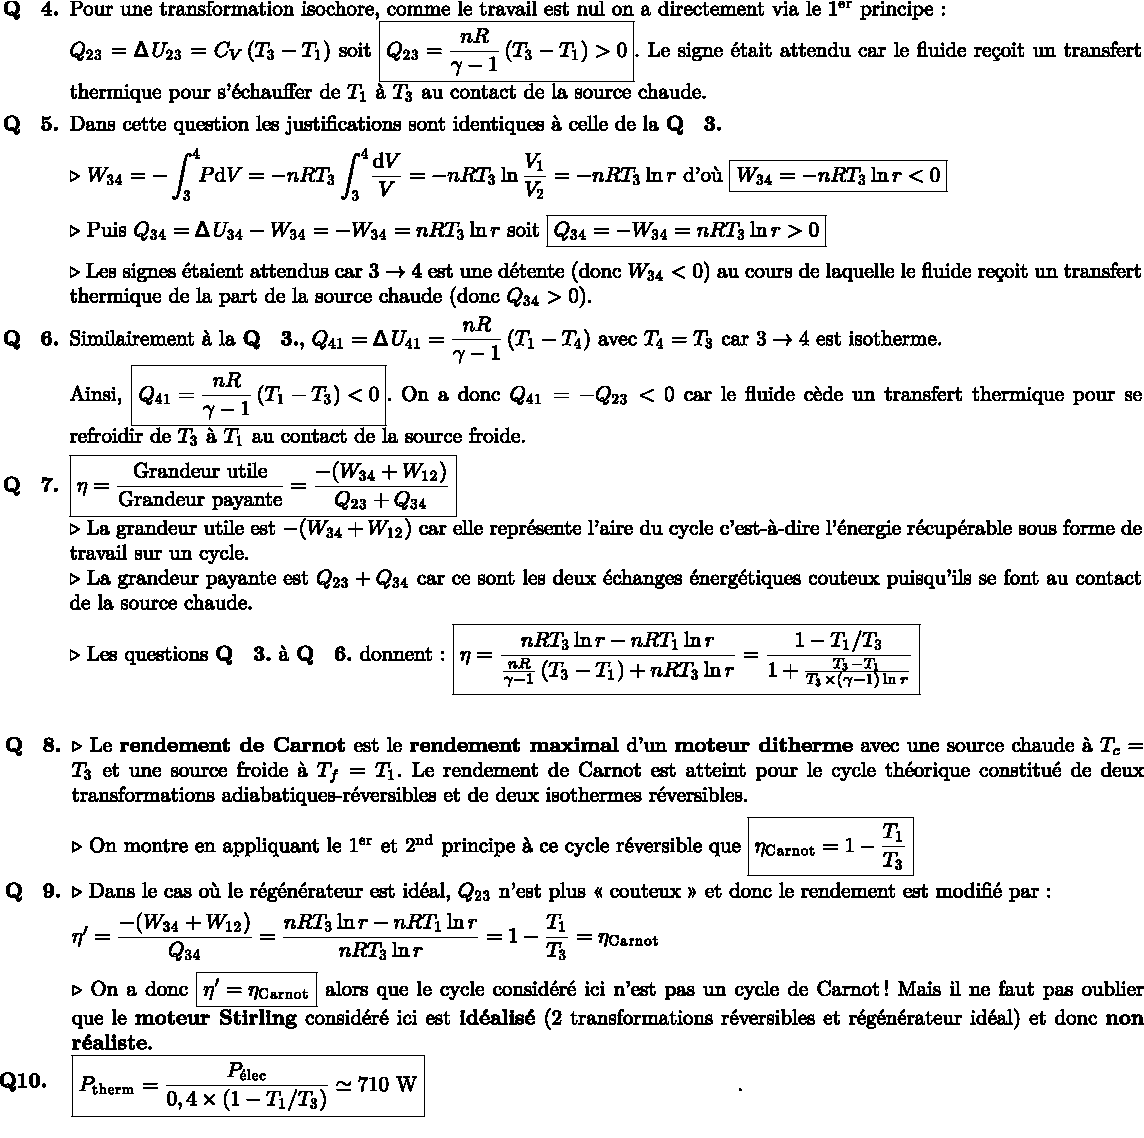
\includegraphics[width=\linewidth]{figures/pb-stirling-corr3.pdf}
\end{center}

\section"P"{Étude thermodynamique d'une chambre froide}

\begin{center}
	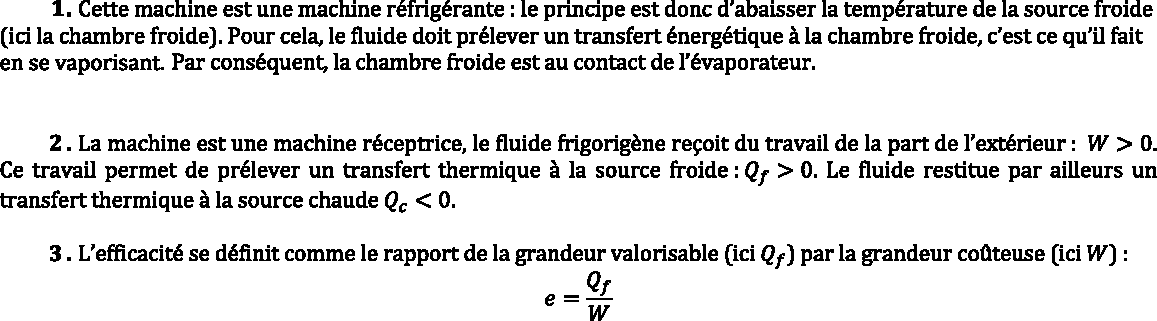
\includegraphics[width=\linewidth]{figures/pb-chambre-corr1.pdf}\\
	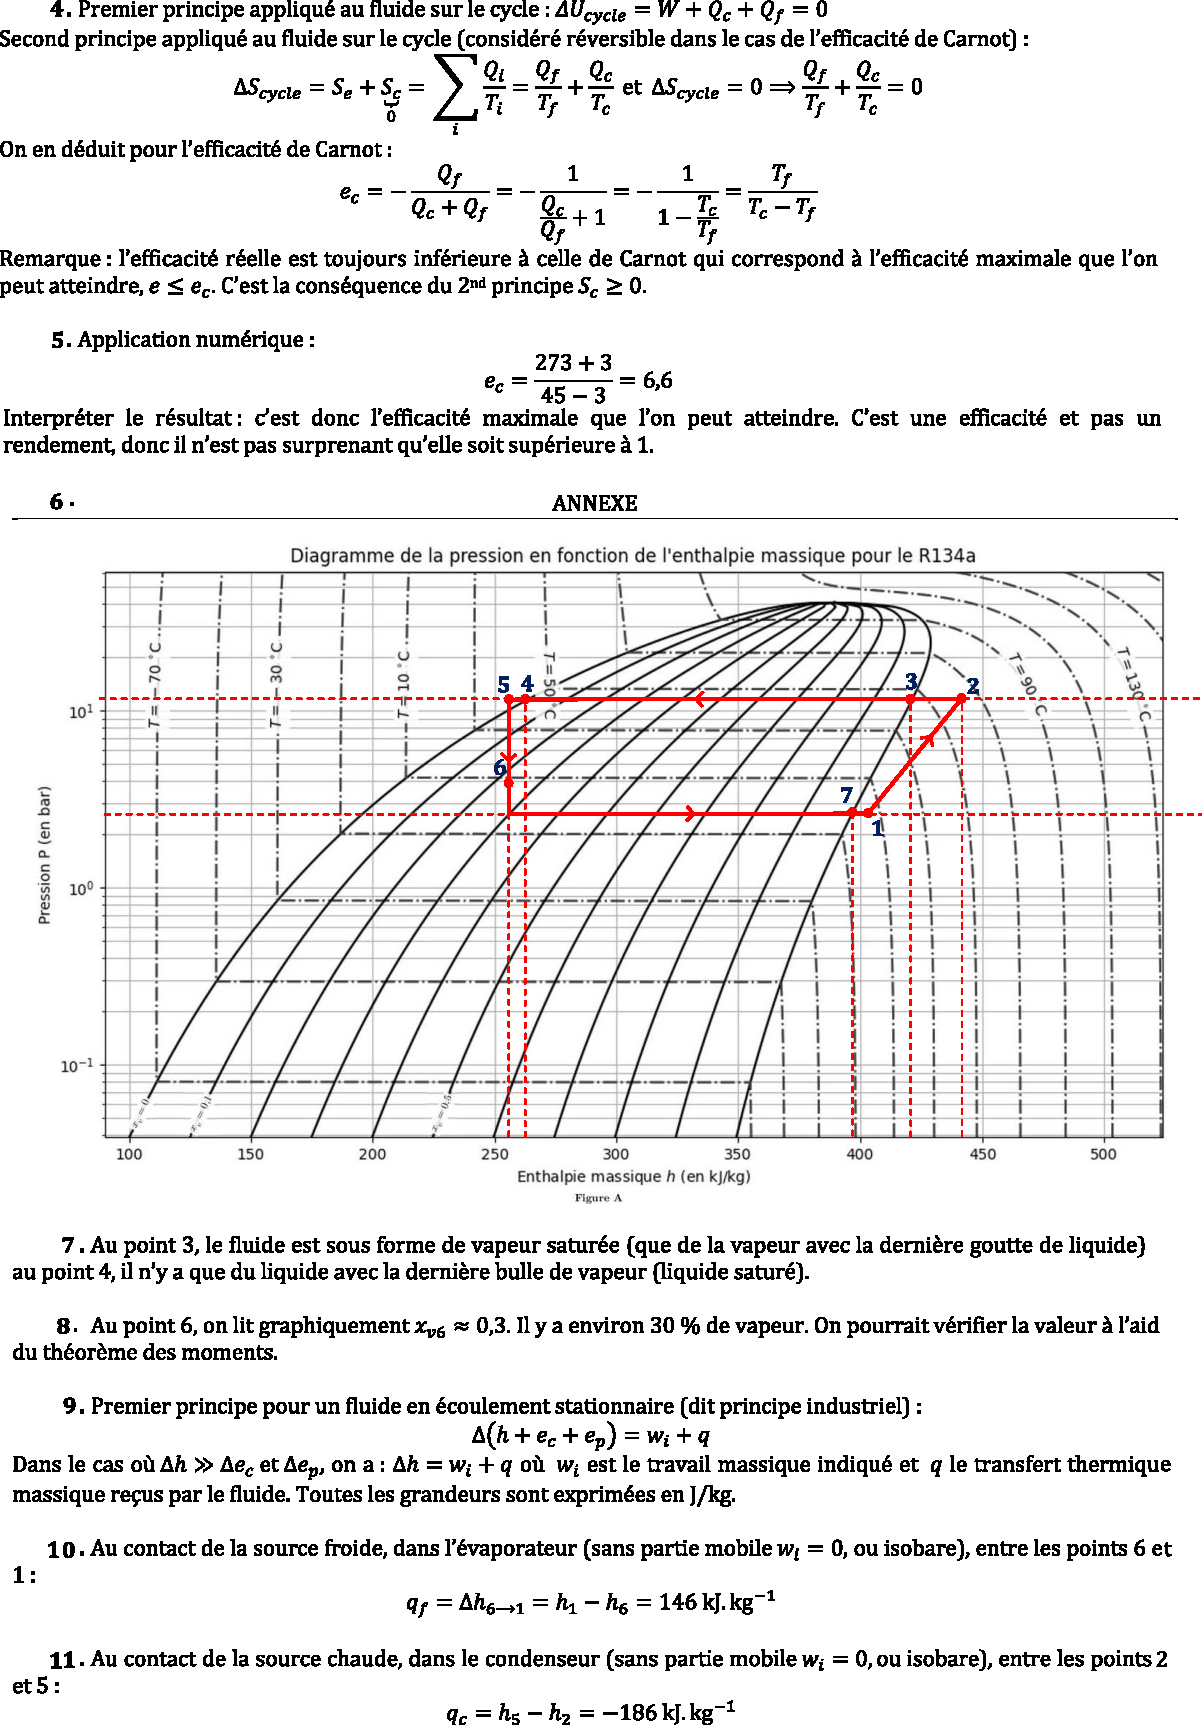
\includegraphics[width=\linewidth]{figures/pb-chambre-corr2.pdf}\\
	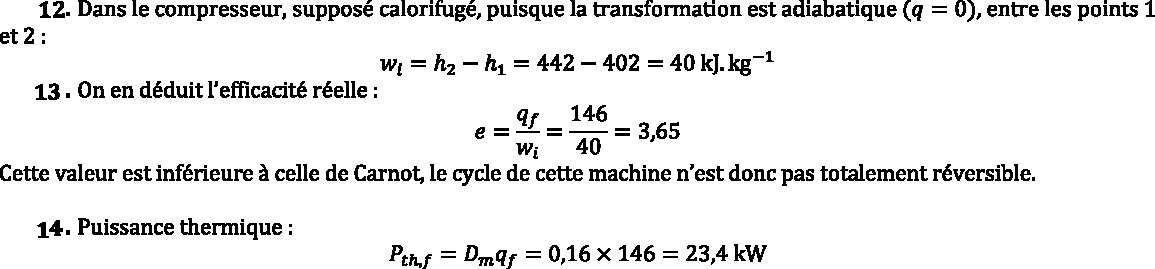
\includegraphics[width=\linewidth]{figures/pb-chambre-corr3.pdf}
\end{center}

\end{document}
